\section{Abstracción y modelado}
El objeto a modelar es una intersección de $N$ calles o avenidas. Con el objeto de profundizar el análisis, se tomará el caso de una intersección de dos avenidas. A lo largo de este trabajo se utilizará el termino \enquote{tramo} para designar al medio por el cual arriban vehículos o personas a la intersección. Una avenida de doble sentido de circulación tiene dos tramos. Con lo cual una intersección de dos avenidas tiene cuatro tramos más un tramo diferenciado para los peatones.

Se asume que se existe una forma fiable de detectar la presencia de vehículos en un tramo. Se dice que un tramo está \enquote{activo} si y solo si hay al menos un vehículo en él.

Por otro lado, también se debe tener en cuenta la presencia de peatones. Para ello se asume que en cada senda peatonal de la intersección hay un pulsador que permite a un peatón solicitar el paso por una de las sendas peatonales. El tramo de peatones se activa con presionar una vez el pulsador y permanece activo hasta ser atendido. Se dice que un tramo es atendido cuando el sistema de semáforos permite el paso de vehículos o personas, es decir, tiene su semáforo correspondiente en verde.

Para simplificar el análisis, se modela a la intersección como un recurso compartido al cual se accede con exclusión mutua. Es decir, la intersección puede ser adquirida a lo sumo por un tramo.

\subsection{Uso de procesos}
Basándose en el marco teórico de la programación concurrente, se puede modelar a cada tramo como un proceso que trata de acceder al recurso compartido (la intersección). De esta forma el problema del control del tránsito se reduce al de la planificación de un recurso compartido. Este recurso compartido programáticamente se convierte entonces en una sección crítica.

\begin{figure}
	\centering
	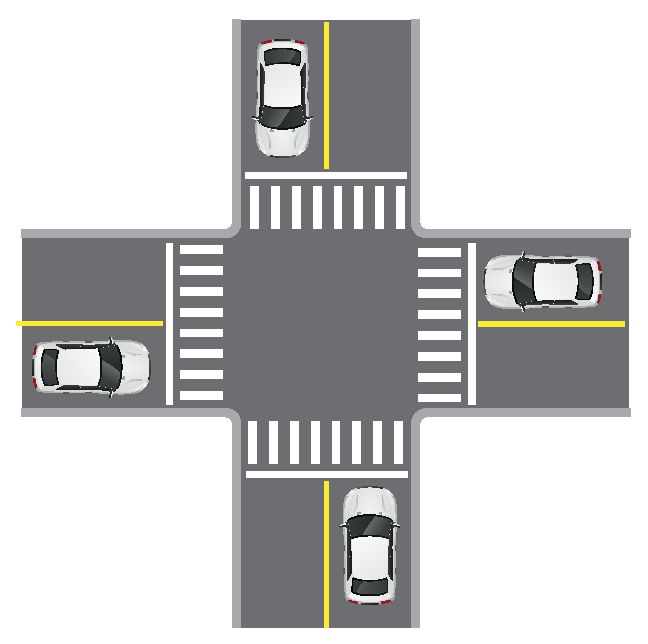
\includegraphics[width=10cm]{imagenes/interseccion-base.eps}
	\caption{Intersección base.}
	\label{fig:interseccion-base}
\end{figure}

\section{Implementaciones}

\section{Implementación A}
\section{Implementación B}
\section{Implementación C}
